In diesem Kapitel wird die Umsetzung der Hardware sowie Firmware des \acrshort{tof}-Demonstrators dokumentiert.

Im Anhang~\ref{sec:schematic_apdx} bis und mit~\ref{sec:apdx_photos_demonstrator} sind sämtliche technischen Dokumente
sowie einige Fotos des fabrizierten Demonstrators abgelegt.

\subsection{Schaltungen}
Nachfolgend werden sämtliche Teil-Schaltungen thematisiert, welche für das entwickelten \acrshort{tof}-Evaluationsmodul
nötig sind. Ein vollständiges Schema kann dem Anhang~\ref{sec:schematic_apdx} entnommen werden. Die kompletten
Projekt-Dateien sind im elektronischen Anhang dieses Projektes verfügbar.

Designt wurde das Schema mit Hilfe des Open-Source Tools \dq KiCad EDA 8.0\dq\ \cite{kicad2025kicadeda}.

\subsubsection{Selective Input Voltage}

Abbildung~\ref{fig:selective_input_voltage} zeigt die Beschaltung zur Selektion der Speisung.

\begin{figure}[H]
    \centering
    \includegraphics[page=2, trim=80 590 750 50, clip, width=0.9\textwidth]{attachments/schematic.pdf}
    \caption{Selective Input Voltage}\label{fig:selective_input_voltage}
\end{figure}

Für die Speisung des Nucleo-Boards bestehen die folgenden Möglichkeiten:

\begin{itemize}
    \item 5~V von USB-Buchse
    \item 5~V von externem Power-Supply (\lstinline|JP1| + \lstinline|JP2|)
    \item 12~V von externem Power-Supply (\lstinline|JP3|)
\end{itemize}

Siehe dazu auch Kapitel~\ref{sec:schematic_nucleo}.

Für die Speisung der 5~V Elektronik bestehen die folgenden Möglichkeiten:

\begin{itemize}
    \item 5~V von Nucleo-Board (\lstinline|JP1|)
    \item 5~V von externem Power-Supply (\lstinline|JP2|)
    \item 12~V von externem Power-Supply via Nucleo-Board (\lstinline|JP1| + \lstinline|JP3|)
\end{itemize}

Für die Speisung der Photodiode bestehen die folgenden Möglichkeiten:

\begin{itemize}
    \item 5~V von 5~V-Elektronik (\lstinline|SW2| Position 3)
    \item 12~V von externem Power-Supply (\lstinline|SW2| Position 1)
\end{itemize}

Siehe dazu auch Kapitel~\ref{sec:schematic_photo_receiver}.

\subsubsection{Nucleo Board}\label{sec:schematic_nucleo}

Die Beschaltung des NUCLEO-F042K6 Boards \cite{st2024nucleof042k6_usermanual} ist in Abbildung~\ref{fig:nucleo_board}
gezeigt.

\begin{figure}[H]
    \centering
    \includegraphics[page=2, trim=530 580 300 50, clip, width=0.9\textwidth]{attachments/schematic.pdf}
    \caption{Nucleo Board}\label{fig:nucleo_board}
\end{figure}

Das NUCLEO Board ist ein sogenanntes \dq Development-Kit\dq, welches eine STM32F042K6 \acrshort{mcu}
beinhaltet. Am Rand des Boards werden diverse Pins der \acrfull{mcu} via Pin-Header
einfach zur Verfügung gestellt. Dies erleichtert die Integration in eine eigene Elektronik
enorm. Programmiert wird die \acrshort{mcu} über eine \acrshort{usb}-Schnittstelle.

In diesem Design wird das Entwicklerboard dazu benötigt, die TDC7200 ICs zu
bedienen. Dazu wird einerseits ein \acrfull{spi} benötigt, um die Mess-ICs zu konfigurieren
und auch auszulesen (siehe SPI-Bus in der Abbildung). Weiter können auf beiden \acrshort{tdc}s Messungen
gestartet werden mit den Signalen \lstinline|start_ele|, resp. \lstinline|start_opt|. Für den
\acrshort{tdc} welcher sich um die elektrischen Signale kümmert kann zudem mit \lstinline|stop_ele| ein
Stopp-Puls generiert werden.
Zu guter Letzt ist das NUCLEO dafür zuständig, die Laser-Diode anzusteuern, was mit den Signalen
\lstinline|LD_pulse| sowie $\overline{\mbox{\lstinline|LD_enable|}}$ geschieht.

\subsubsection{TDC Electrical Signal}

Die Beschaltung des TDC7200 \cite{ti2016tdc7200_datasheet} für den elektrischen Teil ist in
Abbildung~\ref{fig:tdc_ele_signal} gezeigt.

\begin{figure}[H]
    \centering
    \includegraphics[page=2, trim=80 330 750 310, clip, width=0.9\textwidth]{attachments/schematic.pdf}
    \caption{\acrshort{tdc} Electrical Signal}\label{fig:tdc_ele_signal}
\end{figure}

Der TDC7200 ist über die die Start- und Stopp-Leitungen, ein Enable-Signal sowie die \acrshort{spi}-Leitungen mit der
\acrshort{mcu} verbunden.

Wie bereits im Kapitel~\ref{sec:approach} angesprochen, wird der elektrische \acrshort{tdc} dazu verwendet, den Chip
erstmalig in Betrieb zu nehmen und sich damit vertraut zu machen. Am Anschluss \lstinline|J3| kann in einem nächsten
Schritt ein beliebig langes Kabel angeschlossen werden. Dies ermöglicht es, erste Messresultate, natürlich rein elektrisch,
vom TDC7200 auszulesen.

Mittels Schalter \lstinline|SW1| kann das \lstinline|STOP|-Signal wahlweise via \lstinline|stop_ele| oder
\lstinline|start_ele| generiert werden. Dies bietet zum einen die Möglichkeit, die Zeit zwischen dem Schalten von zwei
\acrshort{gpio}s zu messen. Zum anderen, kann derselbe \acrshort{gpio}-Pin zum Generieren des \lstinline|START|- und
\lstinline|STOP|-Signals verwendet werden, wodurch von der Verzögerungszeit direkt auf die Kabellänge an \lstinline|J3|
geschlossen werden kann.

\subsubsection{TDC Optical Signal}

Die Beschaltung des TDC7200 \cite{ti2016tdc7200_datasheet} für den optischen Teil ist in
Abbildung~\ref{fig:tdc_opt_signal} gezeigt.

\begin{figure}[H]
    \centering
    \includegraphics[page=2, trim=530 330 300 310, clip, width=0.9\textwidth]{attachments/schematic.pdf}
    \caption{\acrshort{tdc} Optical Signal}\label{fig:tdc_opt_signal}
\end{figure}

Die Beschaltung des \acrshort{tdc}s für die optische Messung gestaltet sich praktisch gleich wie beim elektrischen
Gegenstück. Der Hauptunterschied ist, hier aber, dass dessen \lstinline|STOP|-Signal nicht von der \acrshort{mcu} selber generiert
wird, sondern von einem Komparator, welcher am Ende des optischen Messpfades steht. Da der Komparator mit einem 5~V Pegel
arbeitet, ist der Spannungsteiler \lstinline|R1| / \lstinline|R2| vonnöten, welcher den 5~V Puls auf die geeigneten 3.3~V
herunterteilt.

\subsubsection{Oscillator For TDCs}

Die Beschaltung des Oszillators für die beiden \acrshort{tdc} ist in Abbildung~\ref{fig:oscillator_tdc} gezeigt. Es
handelt sich hierbei um einen normalen Quartz-Oszillator mit integriertem Schwingkreis. Praktischerweise ist bei diesem
also keine weitere Beschaltung notwendig.

\begin{figure}[H]
    \centering
    \includegraphics[page=2, trim=80 90 930 550, clip, width=0.45\textwidth]{attachments/schematic.pdf}
    \caption{Oscillator for \acrshort{tdc}s}\label{fig:oscillator_tdc}
\end{figure}

\subsubsection{Power Supply Separation}

Für die Beschaltung der Photodiode, inkl. \acrshort{tia} und Komparator, macht es Sinn eine Spannungsversorgung mit
möglichst wenig Rauschen zu haben.

Dazu wurde die Separierung vorgenommen, welche in Abbildung~\ref{fig:power_supply_separation} dargestellt ist.

\begin{figure}[H]
    \centering
    \includegraphics[page=2, trim=260 90 640 550, clip, width=0.7\textwidth]{attachments/schematic.pdf}
    \caption{Power Supply Separation}\label{fig:power_supply_separation}
\end{figure}

Prinzipiell sollen die Speisungen über eine Ferrit-Perle etwas entstört werden. Massgeblich ist hier natürlich auch der
physikalische Verlauf des Speisungspfades auf dem Layout. Dazu mehr im entsprechenden Kapitel~\ref{sec:layout}. Wahlweise
besteht nebst den Ferrit-Perlen die Möglichkeit, mittels Kondensatoren die Speisung weiter zu entkoppeln. Es wird jedoch
davon ausgegangen, dass dies in einem ersten Schritt nicht notwendig ist.

\subsubsection{Laser Driver}\label{sec:schematic_laser_driver}

Die Laser Diode RLD65NZX1 \cite{rohm2019rld65nzx1_datasheet} wird mittels Lasertreiber LMG1025-Q1 \cite{ti2024lmg1025q1_datasheet}
und NexFET \cite{ti2016csd17578q3a_datasheet} angesteuert. Für die Generierung eines kurzen Pulses (0.5 \dots 100~ns)
wurde mittels Hochpass und AND-Gatter \cite{diodes202074lvc1g08q_datasheet} implementiert. Siehe dazu Abbildung~\ref{fig:laser_driver}.

Der Widerstand \lstinline|R25| bildet den Vorwiderstand für die Laser-Diode, welcher sich gemäss der Formel~\ref{eq:ld_resistor} berechnet.

\begin{equation}\label{eq:ld_resistor}
    R_{v} = \frac{V_{cc} - V_{fld}}{I_{ld}} = \frac{5~V - 2~V}{40~mA} = 75~\Omega
\end{equation}

Im Schema eingezeichnet ist aktuell ein Platzhalterwert. Während der Inbetriebnahme wird der Widerstand je nach Bedarf
verändert. Wird dieser beispielsweise verkleinert, so vergrössert sich der Strom durch die Laser-Diode und somit die ausgesandte
Lichtleistung.

%TODO Erwähnen was für ein Widerstand schlussendlich verwendet wurde. z.B. 10x Überansteuerung weil kleiner Duty-Cycle.

\begin{figure}[H]
    \centering
    \includegraphics[page=3, trim=100 520 550 60, clip, width=0.9\textwidth]{attachments/schematic.pdf}
    \caption{Laser Driver}\label{fig:laser_driver}
\end{figure}

\subsubsection{Photo Receiver}\label{sec:schematic_photo_receiver}

Um den Photostrom der Photodiode NJL6401R \cite{jrc2014njl6401r3_datasheet} zu verstärken und in eine Spannung umzuwandeln,
wurde mit dem Operationsverstärker OPA858 \cite{ti2018opa858_datasheet} ein Transimpedanzverstärker aufgebaut. Der
Ausgang des Transimpedanzverstärkers geht auf den Komparator TLV3501 \cite{ti2016tlv3501_datasheet}, um das \lstinline|STOP|-Signal
für den \acrshort{tdc} zu generieren. Siehe dazu Abbildung~\ref{fig:photo_receiver}.

Der Feedback-Widerstand \lstinline|R26| kann je nach bedarf verändert werden. Wird dieser vergrössert, so steigt auch der
negative Puls am Ausgang des \acrshort{tia}s. Mit \lstinline|C20| kann zudem bei Bedarf eine kleine Kapazität hinzugefügt
werden. Diese hat zum Ziel, ein Schwingen des Verstärkers zu unterdrücken, falls dieser eine Neigung zum Schwingen haben
sollte.

Der Offset des OPA858 und die Schaltschwelle des TLV3501 werden mit Hilfe der beiden Trimmer \lstinline|RV22| und
\lstinline|RV23| einstellbar gemacht. Dies hilft bei der Inbetriebnahme, da im Voraus noch nicht ganz klar ist,
wo der Ausgang des Operationsverstärkers aufgrund des gewandelten Dunkelstroms der Photodiode zu liegen kommt.

\begin{figure}[H]
    \centering
    \includegraphics[page=3, trim=100 240 600 340, clip, width=0.9\textwidth]{attachments/schematic.pdf}
    \caption{Photo Receiver}\label{fig:photo_receiver}
\end{figure}

\subsubsection{Decoupling Capacitors}

Die Beschaltung der Entkopplungs-Kondensatoren ist in Abbildung~\ref{fig:decoupling_capacitors} dargestellt. Die
Kondensatoren für den Operationsverstärker OPA858 und für den Komparator TLV3501 wurden dem Vorschlag im Datenblatt
entnommen. Zusätzlich wird auch der Gate-Treiber beim Laser-Treiber mit einer zusätzlichen, grösseren Kapazität gestützt,
was sich positiv auf die Stabilität der Speisung auswirken sollte.

\begin{figure}[H]
    \centering
    \includegraphics[page=3, trim=100 60 650 630, clip, width=0.9\textwidth]{attachments/schematic.pdf}
    \caption{Decoupling Capacitors}\label{fig:decoupling_capacitors}
\end{figure}

\pagebreak

\subsection{Layout}\label{sec:layout}

Beim Layout wurde ein Augenmerk darauf gelegt, dass die verschiedenen Schaltungen sich auf dem \acrshort{pcb} nicht
gegenseitig stören. Dafür wurde ein sauberes Speisungskonzept entworfen, welches die Ground- und Power-Planes nach Layer
definiert. Prinzipiell sind die vier Lagen der Leiterplatte wie folgt aufgetrennt:

\begin{itemize}
    \item Top-Layer: Signal und Ground
    \item Innerer Layer 1: Stromversorgungsebene
    \item Innerer Layer 2: Signal und Ground
    \item Bottom-Layer: Signal und Ground
\end{itemize}

\begin{figure}[H]
    \centering
    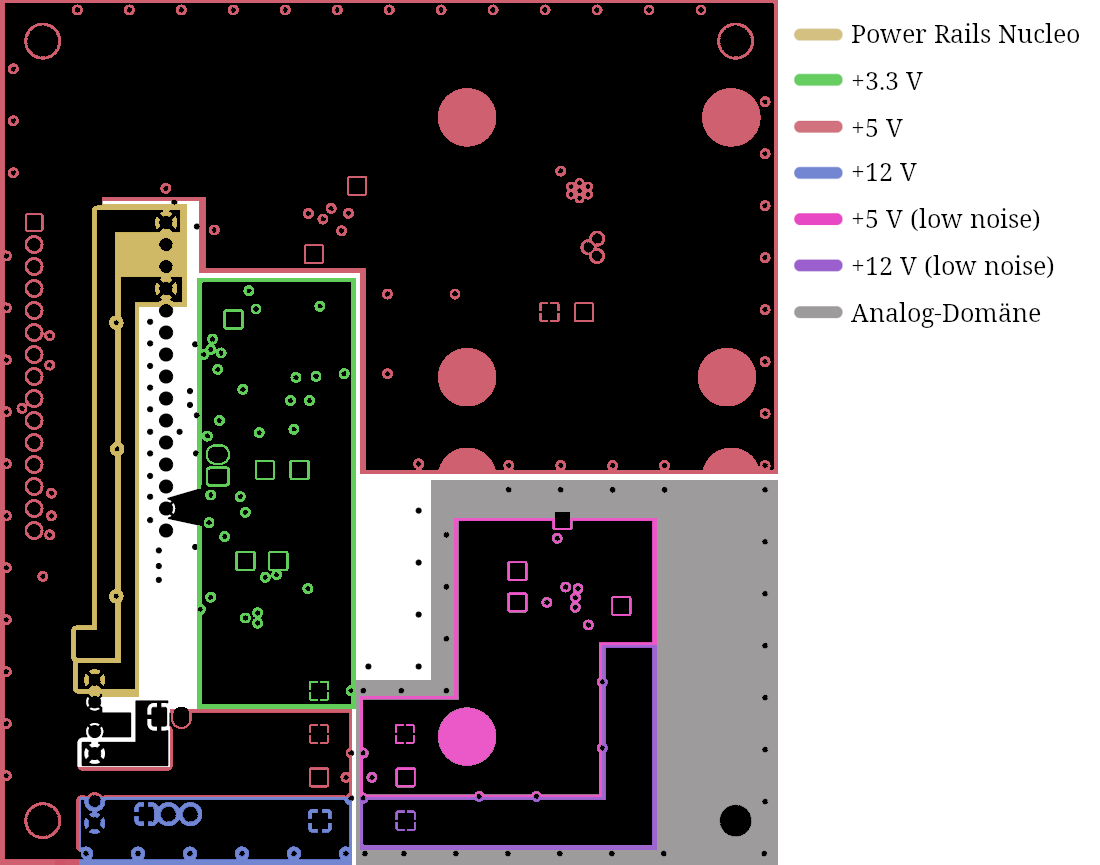
\includegraphics[width=0.9\textwidth]{graphics/layout_annotated.png}
    \caption{Innerer Layer 1 mit Vermerken zum Speisungskonzept}\label{fig:layout_annotated}
\end{figure}

In Abbildung~\ref{fig:layout_annotated} ist die Umsetzung des Speisungskonzeptes ersichtlich. In der unteren, rechten Ecke
befindet sich die Analog-Domäne, welche die Photodiode, den \acrshort{tia} und den Komparator beinhaltet. Dieser Abschnitt
des \acrshort{pcb}s besitzt eigene Ground-Planes sowie entstörte Speisungen. Mit Hilfe von einigen Vias an der Aussengrenze
dieses Abschnittes sollte die Analog-Domäne zudem weniger Anfällig auf extern induzierte Störfelder sein.

Solche sogenannten \dq Stitching-Vias\dq\ sind zudem rund um das ganze \acrshort{pcb} zur Abschirmung platziert.

Das komplette Layout kann dem Anhang~\ref{sec:apdx_layout} entnommen werden.

\pagebreak

\subsection{3D View}
Die 3D-Ansicht wirkte beim Design des Layouts und vor allem bei der Komponentenplatzierung insofern unterstützend, da hier
ersichtlich ist, wo sich mechanische und elektronische Komponenten in den Weg kommen könnten. Die Abbildung~\ref{fig:3d_top}
zeigt eine 3D-Wiedergabe der Aufsicht auf den \acrshort{tof}-Demonstrator.

\begin{figure}[H]
    \centering
    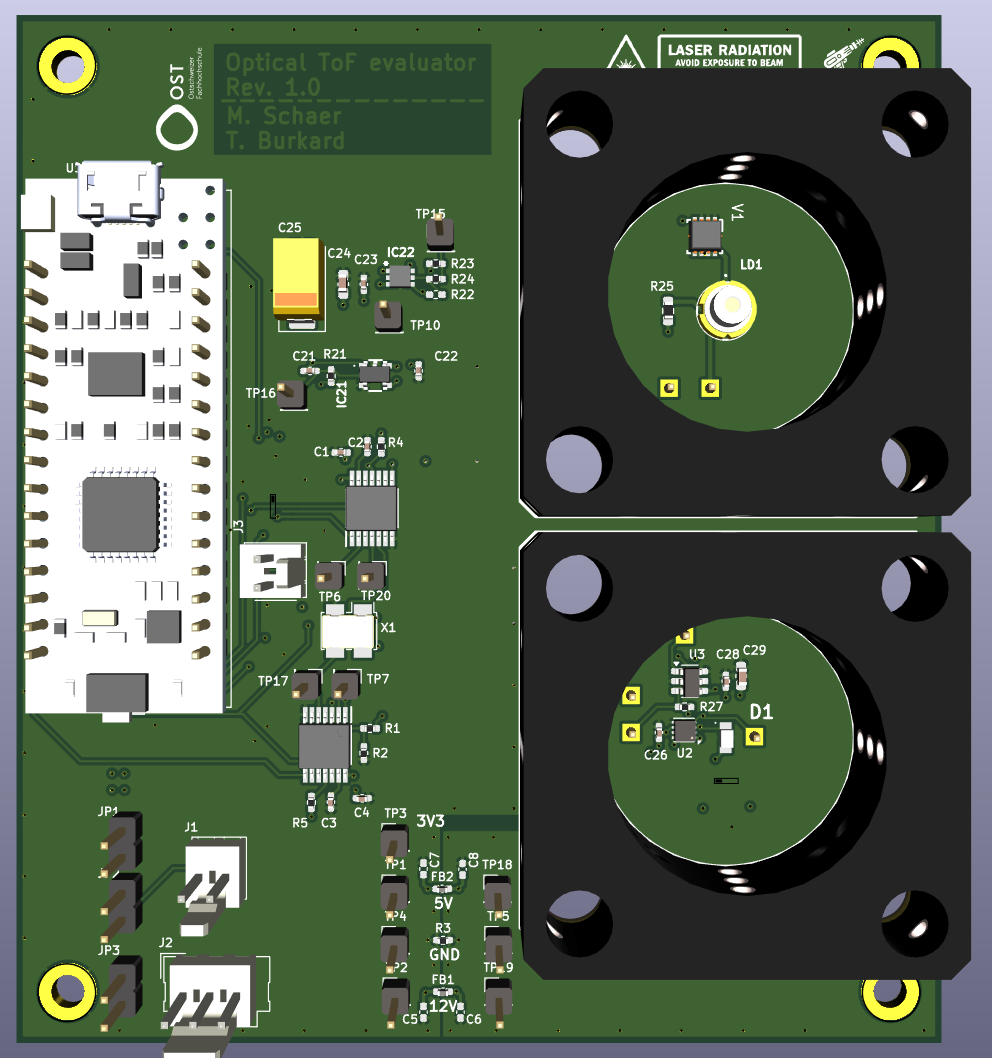
\includegraphics[width=0.5\textwidth]{graphics/3d_top.png}
    \caption{3D View Top}\label{fig:3d_top}
\end{figure}

Die Linsenhalterungen wurden mit Hilfe von einer Step-Datei, die von QIOPTIQ zur Verfügung gestellt wird in die Ansicht
integriert \cite{qioptiq2024g061041000_shoppage}. In der Abbildung~\ref{fig:3d_top} sind diese als schwarze Quader mit
zylinderförmigen Ausschnitten dargestellt. Direkt unter diesen Halterungen dürfen sich keine Komponenten befinden, da
sich die Halterungen ansonsten nicht montieren lassen.

Bei der Komponentenplatzierung wird zusätzlich auch darauf geachtet, dass sämtliche Testpunkte sowie die Trimmer und
Schalter zur Konfiguration gut zugänglich sind. Wenn sich diese Komponenten nahe an den optoelektronischen Komponenten
befinden, wurden sie auf der Unterseite platziert. Somit sind sie auch mit montierter Optik verfügbar.

\subsection{Fabrikation}
KiCad 8.0 ermöglicht es, aus dem Layout-Design diverse Fabrikations-Dateien für die verschiedenen Layer zu erzeugen.
Diese sogenannten Gerber und NC-Drill Dateien können von einem Leiterplattenhersteller zur Produktion einer Leiterplatte
verwendet werden. Wahlweise kann eine Leiterplatte direkt auch bestückt werden, was jedoch zusätzliche Zeit in der Produktion
beansprucht.

Da sich die meisten Komponente auf dem \acrshort{pcb} relativ gut bestücken lassen, wurde auf eine automatisierte Bestückung
verzichtet und die Komponenten wurden von Hand bestückt.

Die Komponenten werden bei Mouser Electronics bestellt, während die Leiterplatten vom chinesischen Hersteller JLCPCB
bezogen werden. Mouser erfüllt die erwartete Lieferzeit von einigen Tagen. Die Bestellung von JLCPCB kam mit genau sieben
Tagen ebenfalls pünktlich an. Die Ingenieure von JLCPCB mussten keine Rückfragen zum Design stellen, was sich wohl positiv
auf die Lieferzeit ausgewirkt hat.

Die fertig bestückte Leiterplatte ist in der Abbildung~\ref{fig:photo_demonstrator_front_wo_lens} ersichtlich. Weitere
Fotografien des \acrshort{tof}-Demonstrators können dem Anhang~\ref{sec:apdx_photos_demonstrator} entnommen werden.

\begin{figure}[H]
    \centering
    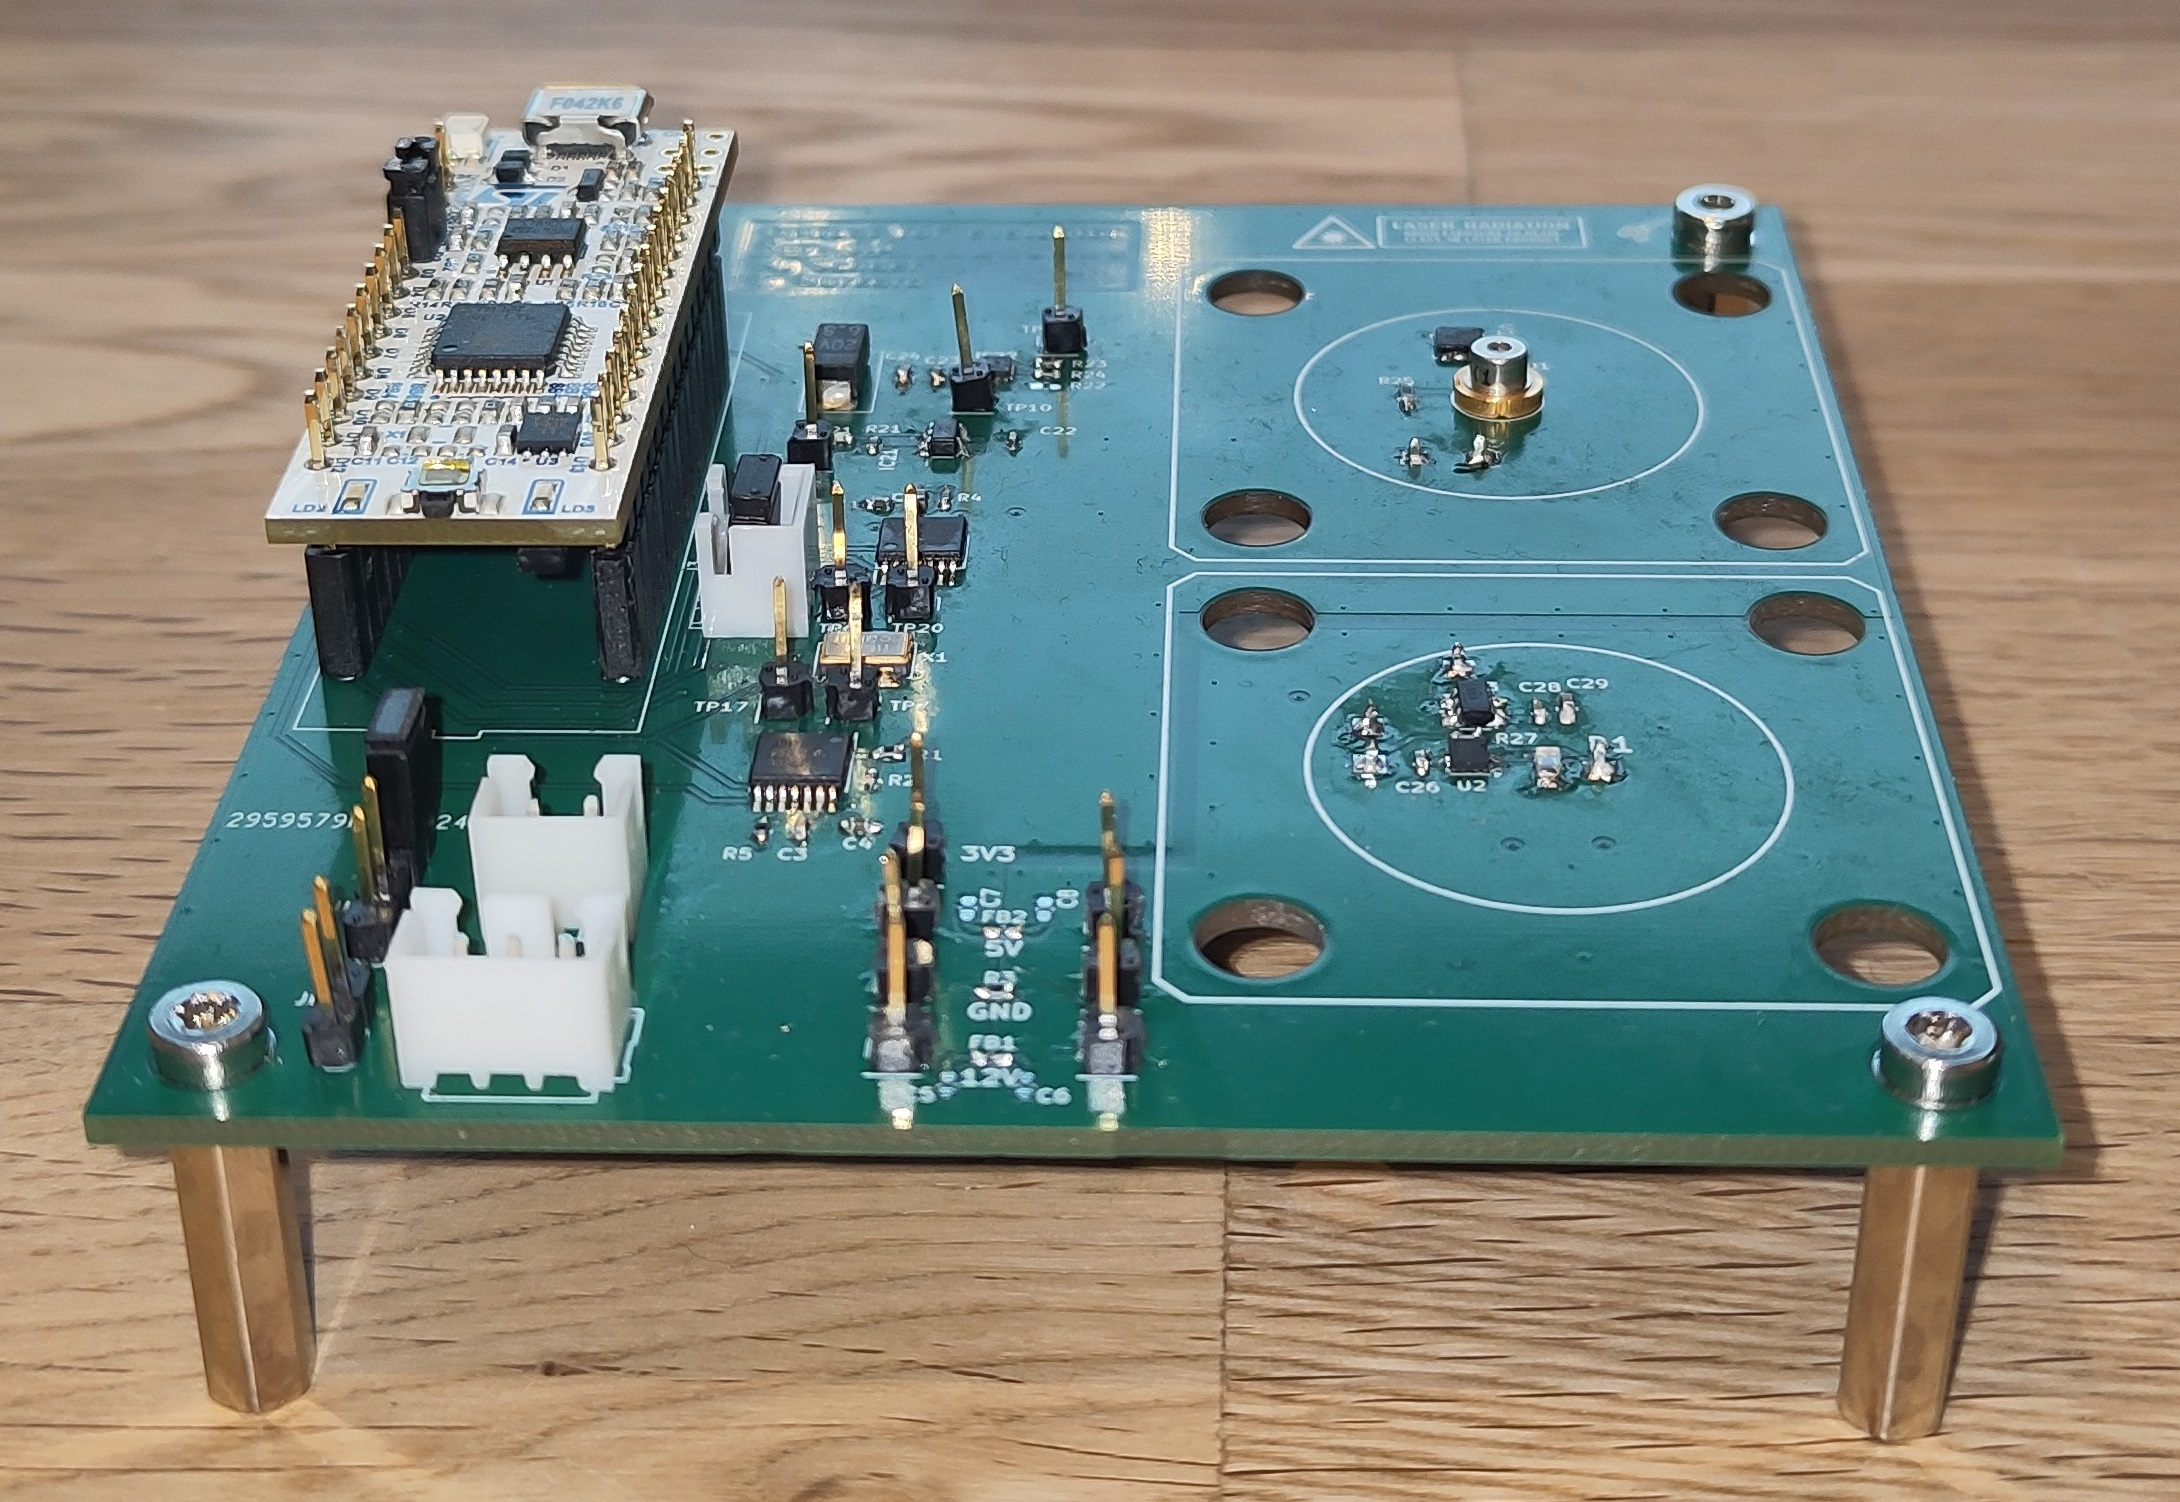
\includegraphics[width=0.6\textwidth]{graphics/photo_demonstrator_front_wo_lens.jpg}
    \caption{Demonstrator von vorne ohne Linse}\label{fig:photo_demonstrator_front_wo_lens}
\end{figure}

\subsection{Firmware}

Bei der Firmware wird ein Augenmerk darauf gelegt, dass es eine saubere Trennung zwischen Applikation, Treiber und
Peripherie gibt. Dies sorgt für ein möglichst modulares Design. Die \acrshort{fw}-Hierarchie ist in der
Abbildung~\ref{fig:hierarchy_firmware} nachvollziehbar.

\begin{figure}[H]
    \centering
    \includegraphics[width=0.5\textwidth]{diagrams/Aufbau_FW.pdf}
    \caption{Aufbau Firmware-Projekt}\label{fig:hierarchy_firmware}
\end{figure}

Die Applikation ist für das Timing der Messungen verantwortlich. Der Code für das auslösen wurde schrittweise ausgebaut,
erst über die Verwendung einfacher \acrshort{gpio}s, bis hin zu optimalem zeitlichen Verhalten unter Einsatz verschiedener
Hardware-Timer für das Generieren der Trigger-Pulse für die \acrshort{tdc}s. Im Kapitel~\ref{sec:electrical_measurements}
sind die einzelnen Erweiterungsschritte detailliert erklärt.

Der \acrshort{tdc}-Treiber beinhaltet die komplete Registerdefinition des TDC7200. Der Treiber stellt zudem einfache Lese- und
Schreib-Routinen zur verfügung, mit Hilfe derer das Mess-\acrshort{ic} mit Leichtigkeit umkonfiguriert, aufgesetzt und
ausgelesen werden kann. Weiter kann der Treiber die Messresultate direkt umrechnen, anhand der im Datenblatt vorgegebenen
Formeln. Im Listing~\ref{code:start_measurement_tdc} ist der Beispiel-Code für eine einzelne Messung ersichtlich.

\lstinputlisting[language={C}, label={code:start_measurement_tdc}, caption={\acrshort{tdc} Messung mit Treiber}]{sourcecode/example_tdc_read.c}

Der selbst entwickelte Firmware-Treiber für den \acrshort{tdc} befindet im Anhang~\ref{sec:tdc_driver}.

Mit Hilfe der Entwicklungsumgebung STM32CubeIDE / CubeMX ist es möglich, das Pinout der \acrshort{mcu} grafisch zu
konfigurieren. Mit Hilfe eines Code-Generators können die Initialisierungs-Routinen für sämtliche Peripherien automatisiert
erzeugt werden. Somit kann während der Entwicklung der Fokus auf den TDC-Treiber sowie die eigentliche Applikation gelegt
werden.

Die Pinkonfiguration ist in der Abbildung~\ref{fig:pinconfiguration_mcu} ersichtlich.

\begin{figure}[H]
    \centering
    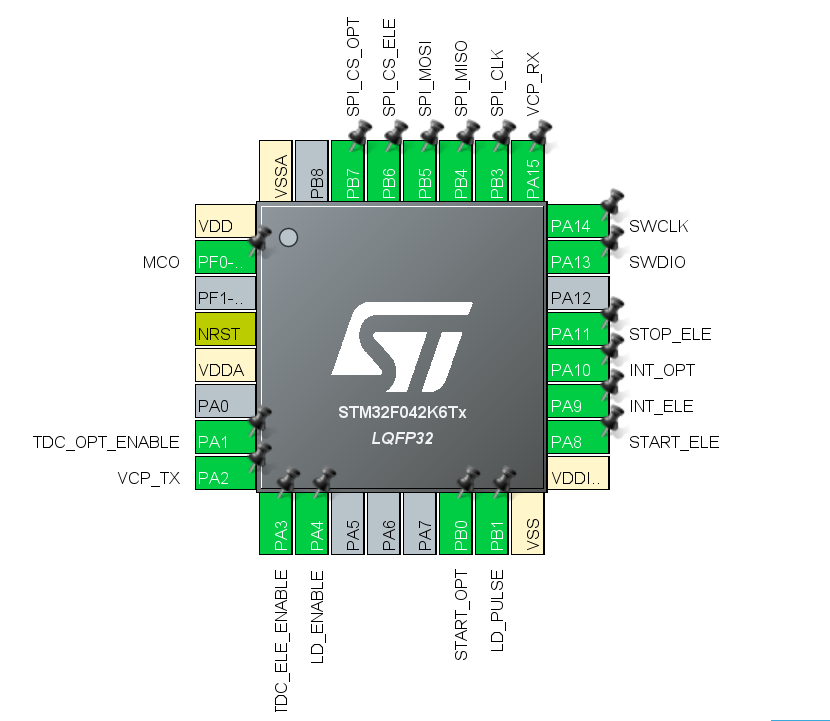
\includegraphics[width=0.6\textwidth]{graphics/pinconfiguration_mcu.png}
    \caption{Pinkonfiguration des STM32F042K6}\label{fig:pinconfiguration_mcu}
\end{figure}

\pagebreak